\section{Preliminary evaluation}
For evaluation, we use 2 platforms: 1)A Raspberry Pi-based Quadcopter running Ardupilot, and 2) Ardupilot-based Quadcopter SITL (Software in the Loop) simulator on an machine running Ubuntu.

For simplicity, we choose anomalies in the position control of the UAV. two kinds of missions are performed -- planar square mission and a vertical lift-off and land. The values of linear position along the three axes are noted at different points of time as shown in the table \ref{fig:data}.

\begin{figure*}[h!]
    \centering
    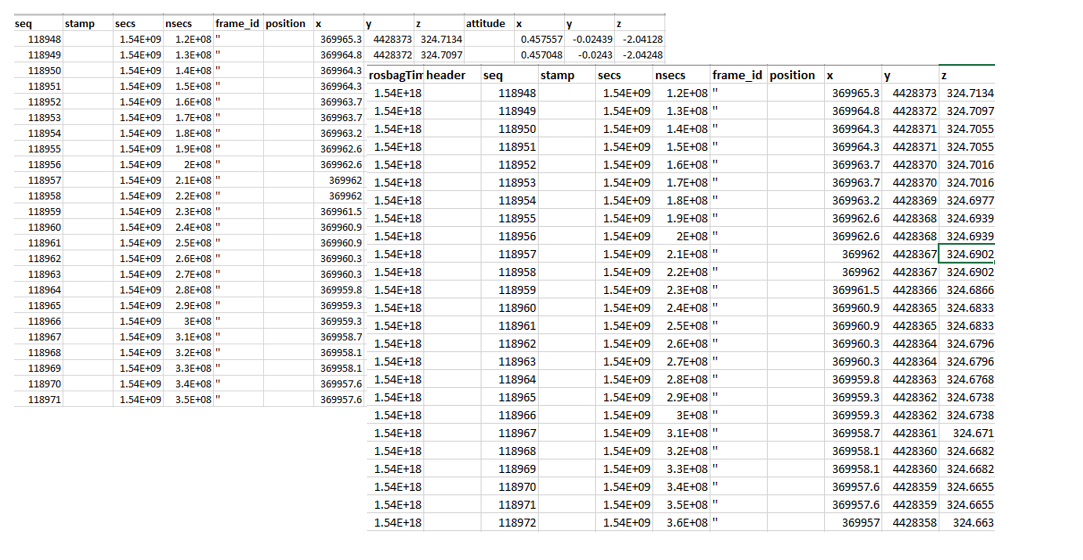
\includegraphics[width=\textwidth]{images/data.png}
    \caption{The values of linear and angular position is noted at different instances of time along the three axes x, y, and z. This is fed into the PID controller to track the error values at different points of time.}
    \label{fig:data}
\end{figure*}

As an example, we get the value of matrix A and B for one of the missions respectively as

$\left({\begin{array}{ccc} 0.7514 & -0.0565 & -0.0248 \\ 0.0758 & 0.9750 & 0.0075 \\ 0.0011 & 0.0025 & 0.9578 \end{array}}\right)$ , and 

$\begin{pmatrix} 1.2545 & 10.5876 & 10.0631 \end{pmatrix}$

The next steps include instrumenting and keeping track of the observed error at the autopilot for each of the missions. This error time series can then be used to develop a statistical test for anomaly detection.  